\documentclass[a4paper,11pt]{article}
\usepackage{indentfirst}
\setlength\parindent{24pt}
\usepackage[T1]{fontenc}
\usepackage[polish]{babel}
\usepackage[utf8]{inputenc}
\usepackage{lmodern}
\selectlanguage{polish}
\usepackage[top=2cm, bottom=2cm, left=1cm, right=1cm]{geometry}
\usepackage{lastpage}
\usepackage{fancyhdr}
\pagestyle{fancy}
\makeatletter
\newcommand{\linia}{\rule{\linewidth}{0.4mm}}
\renewcommand{\maketitle}{\begin{titlepage}
    \vspace*{2cm}
    \begin{center}\LARGE
    Politechnika Warszawska\\
    Wydział Elektryczny\\
    \end{center}
    \vspace{5cm}
    \noindent\linia
    \begin{center}
      \LARGE \textsc{\@title}
         \end{center}
     \linia
    \vspace{0.5cm}
    \begin{flushright}
    \begin{minipage}{5cm}
    \textit{Autor:}\\
    \normalsize \textsc{\@author} \par
    \end{minipage}
    \vspace{5cm}
     \end{flushright}
    \vspace*{\stretch{6}}
    \begin{center}
    \@date
    \end{center}
  \end{titlepage}
}
\makeatother
\author{Grzegorz Kopyt}
\title{Specyfikacja Implementacyjna \\
,,Arbitrage''}
\usepackage{graphicx}
\fancyhf{}
\rfoot{\thepage{}/\pageref{LastPage}}
\begin{document}

\maketitle

\tableofcontents
\vspace{1cm}
\noindent\linia

\section{Wstęp teoretyczny}
Dokument ten dotyczy implementacji programu ,,Arbitrage". Został przygotowany w celu przedstawienia pomysłu na algorytm realizujący znajdowanie korzystnej ścieżki wymiany walut oraz dowolnego arbitrażu. Ponadto dokument informuje o technologiach, w których program będzie zrealizowany, testach jakie powinny zostać przeprowadzone oraz sprzęcie, na którym zostanie wykonany i uruchomiony.
\section{Diagram klas}
\begin{center}
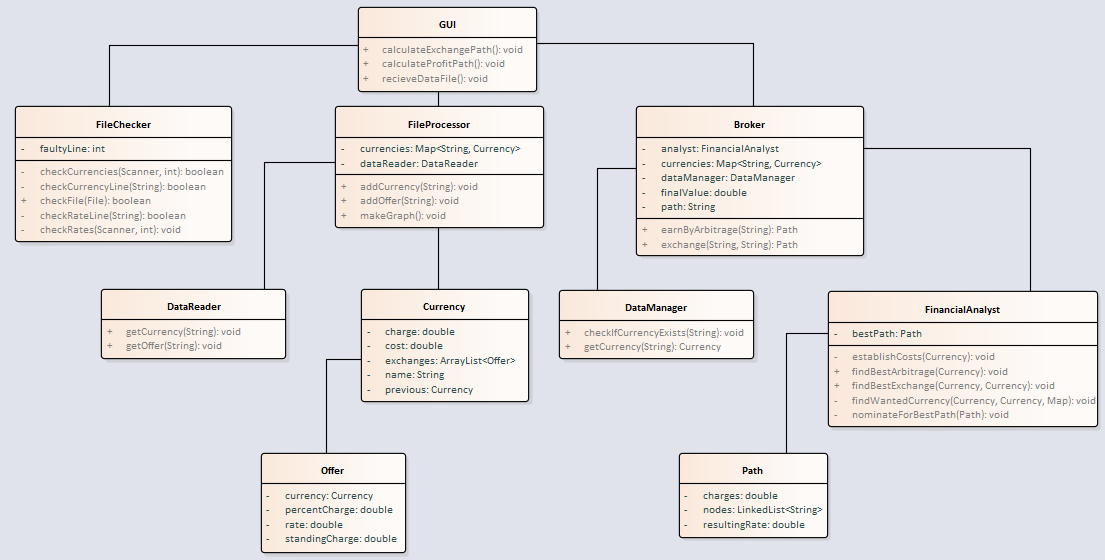
\includegraphics[width = 19cm]{DiagramKlas}
\end{center}

\noindent\linia
\section{Opis algorytmu}

\subsection{Wczytanie danych}

Dane wczytywane będą z pliku tekstowego, wykonanego według wzoru podanym w specyfikacji funkcjonalnej. Plik ten będzie zawierał definicje walut oraz kursy ich wymiany. Na początku zostanie sprawdzony pod kątem zgodności ze wzorem. Jeśli plik będzie wadliwy, algorytm przerwie swoje działanie, a w przeciwnym wypadku będzie kontynuował prace.

Algorytm umieści wszystkie zdefiniowane skrócone nazwy walut w \textit{HashMapie} jako obiekty \textit{Currency}. Dodatkowo każdy obiekt \textit{Currency}, będzie zawierał \textit{Liste} obiektów klasy \textit{Offer}, w których zawarte będą informacje o kosztach i kursie wymiany na inną walutę.

Przykład:
\begin{center}
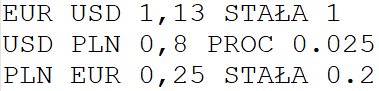
\includegraphics[width = 5cm]{Przyklad}
\end{center}

Obiekt \textit{Currency} reprezentujący walutę \textit{EUR}, będzie zawierał \textit{Liste}, w której będzie obiekt \textit{Offer}.
\\Obiekt \textit{Offer} będzie zawierał:
\begin{itemize}
\item referencję do obiektu \textit{Currency} reprezentującego \textit{USD},
\item informację o kursie wymiany \textit{EUR} na \textit{USD} równym 1.13,
\item informacje o opłacie stałej równej 1,
\item informacje o opłacie procentowej równej 0 (bo jej nie ma w tym przypadku).
\end{itemize} 

Dla innego zestawu danych na tej \textit{Liście} może pojawić się więcej obiektów \textit{Offer} zawierających informacje o wymianie \textit{EUR} na inne waluty.

W ten sposób obiekty \textit{Currency} i ich \textit{Listy} obiektów \textit{Offer} utworzą graf albo wiele grafów w zależności od danych wejściowych i możliwości wymian między walutami.

\subsection{Koszt ścieżki}
Kluczowym zadaniem algorytmu, będzie znajdowanie najkorzystniejszych ścieżek po grafie walut. W celu określenia
\begin{center}
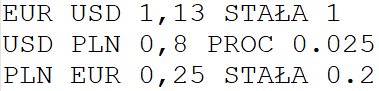
\includegraphics[width = 5cm]{Przyklad}
\end{center}

Koszt dotarcia do danego węzła od wybranego węzła początkowego, będzie przechowywany
Głównym celem jest, aby po skończonej pracy algorytmu w obiektach \textit{Currency} pola \textit{cost} i \textit{charge} miały takie wartości, które kwotę końcową w walucie docelowej pozwolą obliczyć według wzoru:
\\k - kwota początkowa w początkowej walucie
\\w - kwota końcowa w walucie docelowej
\\
\textbf{\emph{w = k/cost - charge}}
\\
\\Wartości pól \textit{cost}, \textit{charge} oraz \textit{previous} w obiektach \textit{Currency} sa zainicjowane wartościami \textit{null}.
\\


Algorytm operuje na grafie, w którym węzłami są obiekty \textit{Currency}, a gałęziami obiekty \textit{Offer}, a jego działanie jest następujące:
\begin{enumerate}

\item Obiekt klasy \textit{Broker} otrzymuje od \textit{GUI} informacje jakie zadanie ma zrealizować i na jakich walutach operować. Są dwa warianty pracy: \textit{wymiana waluty}(patrz 2a.) lub \textit{arbitrage}(patrz 2b.).
\item
\begin{enumerate}
\item Wymiana waluty

\begin{enumerate}
\item \textit{Broker} zleca \textit{FinancialAnalyst}, aby ustawił koszty odwiedzenia węzłów w grafie zaczynając od podanej przez użytkownika waluty wyjściowej.
\begin{enumerate}
\item Z HashMapy \textit{currencies} pobiera Set kluczy, z którego robi tablicę, kluczy.
\item Zaczynając od węzła początkowego iteruje po tablicy w pętli (jeśli napotka koniec tablicy zaczyna od początku).
\item Ustawia \textit{cost} i \textit{charge} węzła początkowego na 0.
\item Ustawia wartości pól \textit{cost} i \textit{charge} w węzłach sąsiadujących z węzłem początkowym według wzorów:
\\
\\\textbf{Cost:}
\\\textit{newCost} - wartośc pola \textit{cost} w sąsiadującym węźle
\\ \textit{cost} - wartość pola \textit{cost} w obecnym węźle
\\ \textit{rate} - wartość pola \textit{rate} w gałęzi \textit{Offer}
\\ \textit{percent} - wartość pola \textit{percentCharge} w gałęzi \textit{Offer}
\\
\\ \textbf{\emph{newCost = cost/rate * (1-percent)}}
\\
\textbf{\\ UWAGA! Jeśli wartość \textit{cost} wynosi zero to:}
\\ \textbf{\emph{newCost = rate * (1-percent)}}
\\
\\\textbf{Charge:}
\\\textit{newCharge} - wartośc pola \textit{charge} w sąsiadującym węźle
\\ \textit{charge} - wartość pola \textit{charge} w obecnym węźle
\\ \textit{rate} - wartość pola \textit{rate} w gałęzi \textit{Offer}
\\ \textit{standingCharge} - wartość pola \textit{standingCharge} w gałęzi \textit{Offer}
\\
\\ \textbf{\emph{newCharge = charge/rate + standingCharge }}
\\
\\\textbf{Wartość \textit{previous} sąsiadującego węzła ustawiamy na obecny węzeł.}
\\
\textbf{\\ UWAGA! Powyższych operacji dokonujemy, jeśli nowa wartość pola \textit{cost} jest mniejsza od poprzedniej.}
\\
\item  Następnie przechodzimy do kolejnego obiektu \textit{Currency} w tablicy:
\begin{itemize}
\item Jeśli wartość jego pola \textit{cost} wynosi \textit{null} to przechodzimy do kolejnego obiektu w tablicy powtarzając podpunkt E.
\item Jeśli wartość jego pola \textit{cost} jest różna od \textit{null} to powtarzamy czynności z podpunktów D, a potem E.
\end{itemize}
\end{enumerate}
\item Teraz aby podać najkrótszą drogę do waluty z waluty podanej wcześniej wystarczy wejść w walutę docelową i prześledzić szlak previous :) warto dodać na początek sprawdzenie na jaką walutę ustawiony jest graf, może nie będzie trzeba liczyć.
\end{enumerate} 
\item Arbitrage
\end{enumerate}
\end{enumerate}

\noindent\linia
\section{Diagram rozwiązania problemu}


\noindent\linia
\section{Opis ważniejszych metod}
\begin{itemize}
\item boolean \textbf{establishCosts}(waluta początkowa)
\\\\
Metoda ustawia w węzłach (Currencies) koszt dotarcia do tego węzła, wyruszając z węzła waluty początkowej. Działa według algorytmu Bellmana-Forda.
Dodatkowo w każdym węźle zostawia informacje, która waluta jako ostatnia zaktualizowała koszt w danym węźle.
\end{itemize}

\noindent\linia

\section{Testy}
\begin{itemize}
\item \textbf{establishCosts}()
\begin{itemize}
\item Metoda dostaje walutę, której nie ma w Mapie. Powinna zwrócić \textit{false}.
\item Metoda dostaje \textit{null}. Powinna zwrócić \textit{false}.
\item Metoda dostaje walutę, która nie ma, żadnego połączenia z innymi. Powinna zwrócić true, a jej pola charge i cost powinny zawierać wartość zero.
\item Metoda dostaje walutę, która ma połączenia z trzema innymi walutami. Powinna zwrócić true i zmienić zawartości pól tych walut.
\end{itemize}
\end{itemize}

\noindent\linia
\section{Informacje o sprzęcie i oprogramowaniu}

\noindent\linia

\end{document}



